\chapter{Results}

\section{Introduction}
Since we believe that using a cognitive architecture will allow for much
more human-like agents, which will lead to engaging and interesting gameplay, we
chose to base our architecture in the global workspace theory, and on the
CERA-CRANIUM model of implementation.

\section{Architecture}
\subsection{Overview}
See figure \ref{fig:our-architecture} for a high-level overview of the
different parts of our architecture. It is highly inspired by the CERA-CRANIUM
architecture. We have some different naming in our figure to make the
distinction of the layers clearer, and also make the placement of the various
processes clearer.

\begin{figure}[h!tb]
\centering
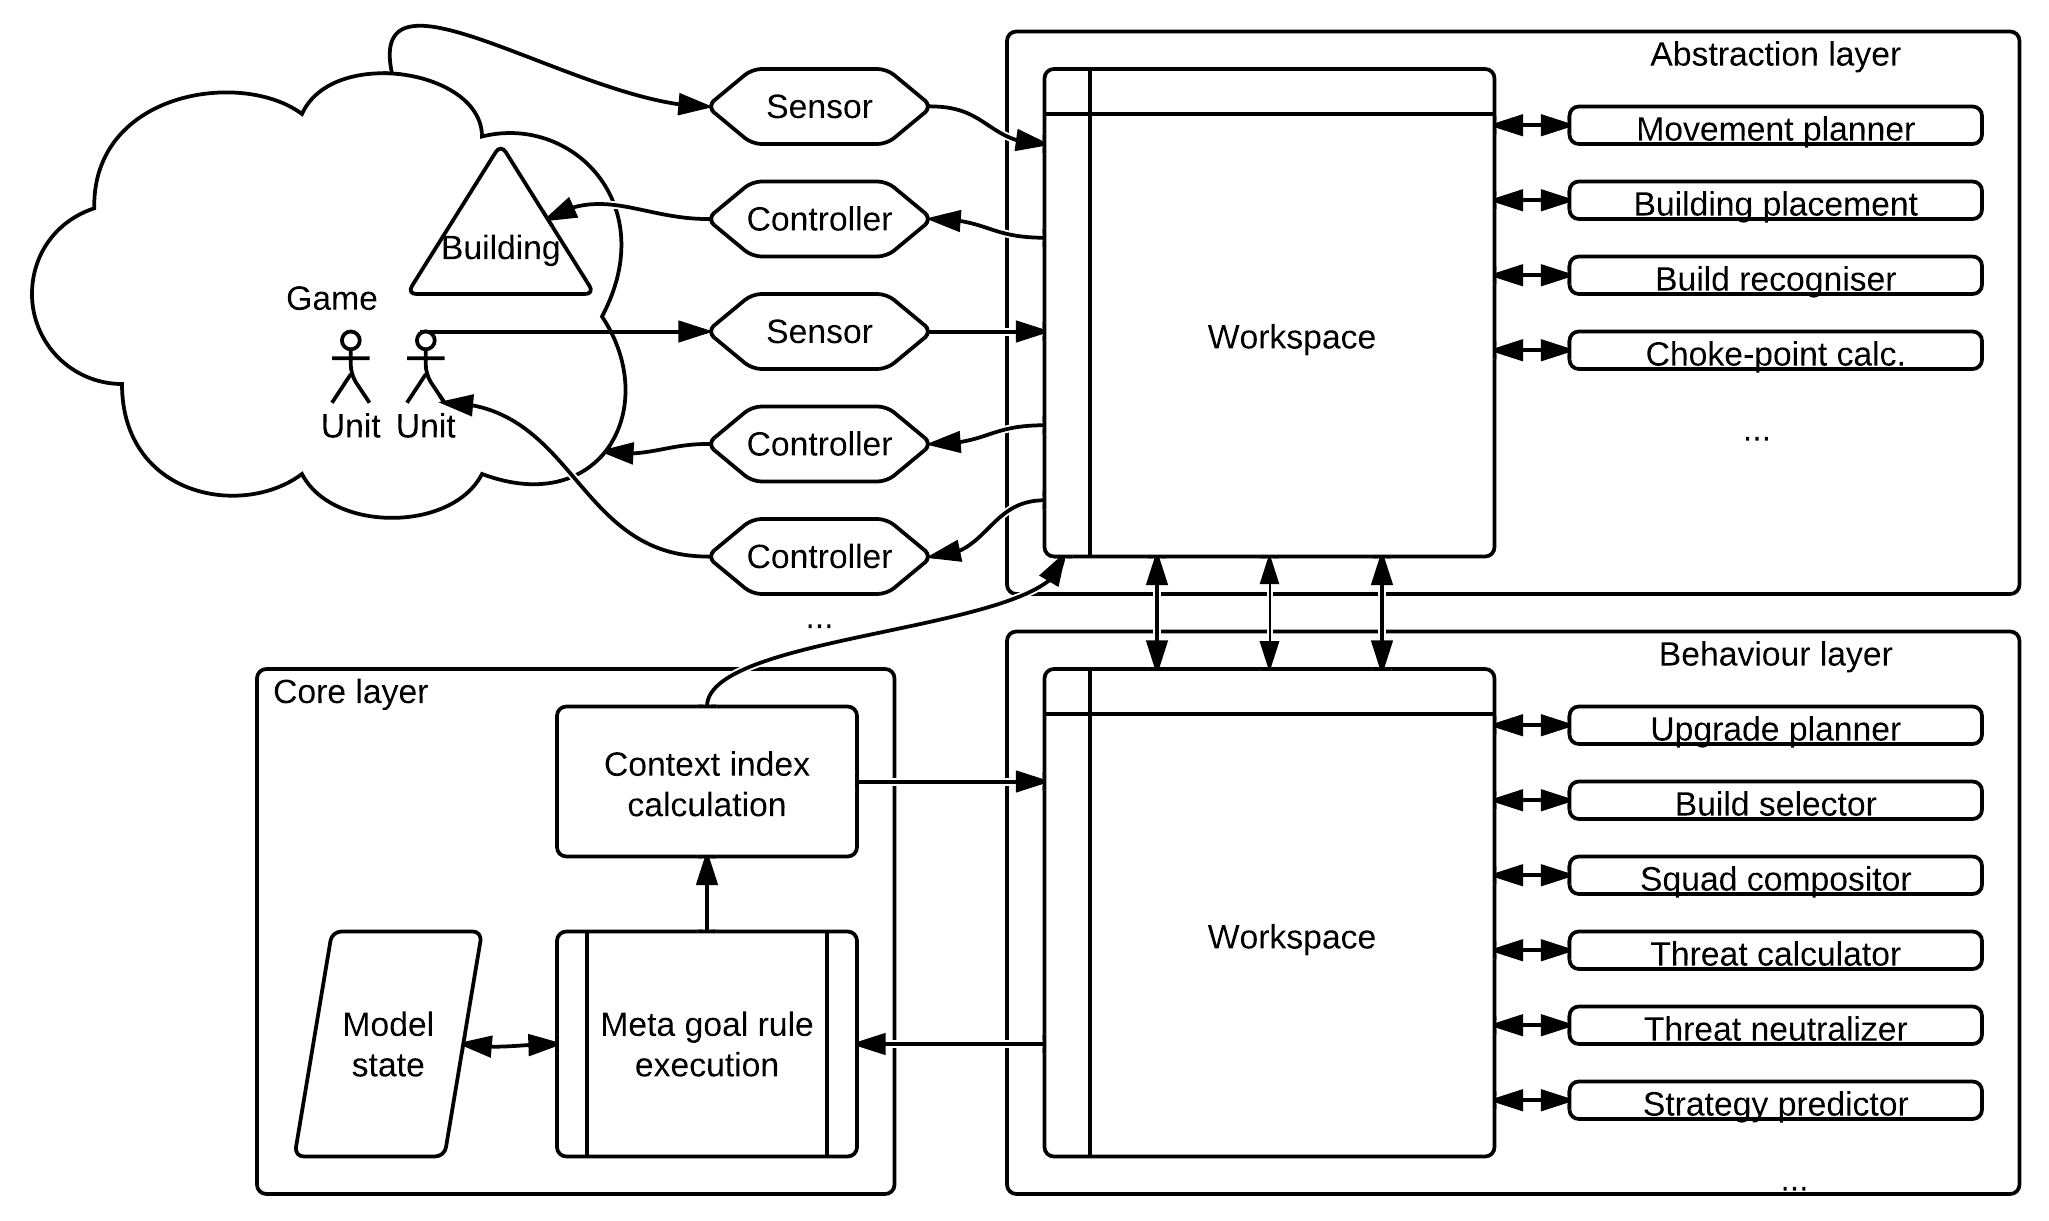
\includegraphics[scale=1.0]{graphics/our-architecture.png}
\caption{High-level model of our architecture}
\label{fig:our-architecture}
\end{figure}

\subsection{The Game}
This ``layer'' is the actual game state, which we interact with through BWAPI.
It approaches a physical world, although the simulation is not very detailed or
realistic.

\subsection{Sensors and controllers}
These are what allows us to observe and control the game.

We suggest simply wrapping the Event objects received as sensor percepts. The
full list of event types are as follows:
\begin{itemize}
    \item MatchStart
    \item MatchEnd
    \item MatchFrame
    \item SendText
    \item ReceiveText
    \item PlayerLeft
    \item NukeDetect
    \item UnitDiscover
    \item UnitEvade
    \item UnitShow
    \item UnitHide
    \item UnitCreate
    \item UnitDestroy
    \item UnitMorph
    \item UnitRenegade
    \item UnitComplete
    \item SaveGame
    \item None 
\end{itemize}
From this list we can see that at least the Unit-related events, as well as the
NukeDetect event, are highly relevant percepts. The rest are more relevant to
detect game conditions and not directly relevant to the agent.

In addition we suggest using the state of each observable unit as a percept.
This includes position, health and which team it belongs to, as well as the
state of any special abilities. Polling this as well as other information that
we don't receive information for will have to be done periodically, and then
one can generate a percept when the value changes noticeably.

Controllers we suggest be at the level of individual units and buildings. There
will probably have to be specialized controllers for most kinds of units, as
well as for the different kinds of buildings.

\subsubsection{Abstraction layer}
The processes here are responsible for turning the raw sensor percepts into
more usable information for the decision making processes higher up, for
example by doing terrain analysis to be able to detect choke points that need
to be defended. A more advanced process here would be something that looks at
scouted buildings, and tries to map this over knowledge about build orders.

Processes here are also responsible for breaking up the decisions and behaviours
made higher up down into more manageable pieces, as well as executing them step
by step (this includes path-finding), and finding optimal positions for
buildings.

An important aspect here is squad movement and handling. This includes
micro-managing units so that they are positioned optimally (units with high
armor and without ranged attacks should be in front, for example, while
vulnerable units with ranged attacks should be further away from ``hot spots''
and enemy units).

\subsubsection{Behaviour layer}
Processes in this layer are responsible for executing the various kinds of
behaviours on a relatively high level. This includes the basics of selecting
what kind of build orders to go for, how to expand through the tech-tree, what
kinds of units should be grouped together in what squads, and so forth.
Selecting various strategies for micro management might also be implemented here
(maneuvers or special tactics, such has hit-and-runs\footnote{Attacking and
immediately retreating.}, shoot-and-scoots\footnote{Long-range attacks, and
immediately moving before enemy forces arrive.}, overwatch\footnote{One group of
units supporting another group.}, kiting \footnote{Shooting while moving and
keeping distance, usually against enemy forces with inferior range and speed,
allows you to attack enemy units while denying counter-attack}, etc.). The
responsibility of actually executing these moves belongs in the abstraction
layer, however.

Another important aspect here is assessing threats. Because this cognitive
approach restricts us to focus on individual parts of the map, we need to make
sure we aren't oscillating between hot points on the map, while ignoring
several other important ones who are lower rated. One approach to
solving this is to mark threats as ``being dealt with'' when we have selected
and dispatched a response to a threat. This could possibly be integrated into a
single module in the behaviour layer, ``acknowledge-dispatch''.

An important process is opponent modelling, or strategy prediction. It can take
in information about scouted technology and structures, and try to predict what
the opponent is trying to do, using domain specific knowledge and resource
constraints, as well as for example learned knowledge from earlier games.
Mismatches between expected and actual results from this can be represented as
mismatch percepts.

\subsubsection{Core layer}
We propose using a similar rule-based system as described in CERA-CRANIUM for
representing the meta-goals.

Meta goals that could be implemented are emotions such as curiosity and a
desire to dominate the game, as well as a desire for accumulating resources.
This will guide the behaviour of the lower layers, and the interplay between
these will have to be finely tuned to get a good balance between economy and
military power, defenses and offensive tactics.

If the balance is skewered here it could lead to oscillating behaviour and
resource starvation for processes that aren't included in the hot spots
selected by the most active rules.